\section{Метод конечных разностей во временной области}
\label{section:CoreMethod}

\emph{Метод конечных разностей во временной области} (\emph{FDTD}) --- это
популярный численный метод моделирования электромагнитных полей. Он относительно
прост для понимания и реализации. Так как метод работает во временной области,
то он годится для решения задач в очень широком диапазоне частот.

Этот метод относится к общему классу сеточных методов решения дифференциальных
уравнений. В рамках этого метода уравнения Максвелла подвергаются дискретизации
с использованием центрально-разностной аппроксимации как по временной, так и по
пространственным координатам. Полученные конечно-разностные уравнения решаются
программными или аппаратными средствами в каждой точке временной сетки, причем,
компоненты вектора напряженности магнитного поля смещены на половину шага
дискретизации относительно компонент вектора напряженности электрического поля.
Расчет полей в ячейках сетки повторяется до тех пор, пока не будет получено
решение поставленной задачи в интересующем промежутке времени.


\subsection{Возникновение и развитие}

Базовый алгоритм метода был впервые предложен американским ученым Кейном Йе
(англ. Kane Yee) из Калифорнийского университета в~\cite{bib:Yee1966}. Однако,
само название «Finite-difference time-domain» и аббревиатура «FDTD» были даны
методу Алленом Тефлавом (англ. Allen Taflove) из Северо-западного университета
штата Иллинойс. Однако отсутствие мощных электронно-вычислительных машин привело
к тому, что
значительный импульс в развитии и применении метод получил лишь к началу 80-х.
В настоящее время метод FDTD интенсивно развивается, существует множество
дополнений к базовому алгоритму, значительно расширяющих область его приложений.
Некоторые из этих дополнений будут подробно описаны далее в работе.

\begin{chronology}

\item[1966~г.]
Йе разработал базовый алгоритм и вывел базовые уравнения~\cite{bib:Yee1966}.

\item[1975~г.]
Тефлав и Бродвин разработали критерии стабильности для алгоритма, разработанного
Йе. Были получены первые решения двумерных и трехмерных задач на взаимодействия
электромагнитной волны с веществом и первые биоэлектромагнитные
модели~\cite{bib:TafloveBrodwin1975}.

\item[1977~г.]
Холланд, Кунц и Ли применили алгоритм для решения
EMP-проблем~\cite{bib:KunzLee1978part1,bib:KunzLee1978part2}.

\item[1980~г.]
Тефлав ввел аббревиатуру FDTD и опубликовал первый проверенный расчетный
результат (моделировалось проникновение электромагнитных полей в металлическую
трехмерную полость)\cite{bib:Taflove1980}.

\item[1981~г.]
Мур опубликовал первое стабильное граничное условие поглощения второго
порядка~\cite{bib:Mur1981}.

\item[1984~г.]
Ляо разработал улучшенное условие поглощения, основанное на
пространственно-временной экстраполяции полей смежных с границей счетного
объема ячеек~\cite{bib:Liao1984}.
\end{chronology}

\noindent
Затем последовало множество работ, предлагающих усовершенствование метода.
Кроме того, важно понятие граничных условий на основе идеально сочетающихся
слоев (PML), которые были впервые разработаны в 1994~г. Жаном-Пьером
Беренже~\cite{bib:Berenger1994} для двумерного случая и были распространены
Кацем на трехмерный случай.

Примерно с 1990~г.\ метод конечных разностей стал основным для численного
решения многих научных и инженерных задач, связанных со взаимодействием
электромагнитных волн с веществом. Он может быть с успехом применен для решения
широкого спектра задач: от моделирования сверхдлинных электромагнитных волн
в~геофизике (включая процессы в ионосфере) и микроволн (например для изучения
сигнатурной радиолокации, расчета характеристик антенн, разработки беспроводных
устройств связи, в том числе цифровых) до решения задач в оптическом диапазоне
(фотонные кристаллы, наноплазмоника, солитоны и биофотоника). К 2006~г. число
публикаций, посвященных FDTD, достигло двух тысяч. В~настоящее
время 27 компаний разработали коммерческие программы, использующие метод
конечных разностей. Также существует 8~проектов с открытым исходными кодам
и 2~бесплатных с закрытым кодом, предназначенных только для некоммерческого
использования.
Более полный их список можно найти в~источнике~\cite{bib:WikipediaFdtdArticle}.


\subsection{Принципы работы}

Рассматривая уравнения Максвелла, легко заметить, что изменение электрического
поля во времени (частная производная по времени) зависит от изменения магнитного
поля в пространстве (ротора магнитного поля). Поэтому, в каждой точке
пространства значение вектора электрического поля в каждый момент времени
зависит от его значения в предыдущий момент времени и от изменения распределения
вектора напряженности магнитного поля в пространстве.

В то же время, из аналогичных рассуждений можно заключить, что значение
вектора~$\vect{H}$ в каждый момент времени зависит от его значения в предыдущий
момент времени и от изменения распределения вектора~$\vect{E}$ в пространстве.
В памяти компьютера хранятся значения векторов~$\vect{E}$ и~$\vect{H}$
в~каждой ячейке сетки, значения которых пересчитываются с каждой итерацией процесса по времени.

Написанное выше справедливо как для одномерного и двумерного случаев, так и для
трехмерного. Если задача поставлена в нескольких измерениях, то численный
расчет ротора полей сильно усложняется. Поэтому для упрощения расчетов в~методе
FDTD сетки электрического и магнитного поля сдвинуты друг относительно друга
так, что магнитное поле расчитывается в точках, расположенных ровно между
точками, в~которых расчитывается электрическое поле, и наоборот. Эта схема,
известная теперь под названием \emph{сетки Йе}, зарекомендовала себя как очень
надежная и в настоящее время составляет основу большинства современных
реализаций метода FDTD. Рисунок~\ref{fig:YeeCell} иллюстрирует вышесказанное.

Более того, Йе также предложил аналогичную схему для нахождения временных
производных: $\vect{E}$- и $\vect{H}$-компоненты сетки разделены во времени
половиной шага дискретизации.


\subsection{Использование}

Для использования метода необходимо задать счетную область.
\emph{Счетная область} (или \emph{счетный объем}) --- это та область
пространства, в пределах которой выполняется численное моделирование.
Счетным объемом также называется объем счетной области.

В каждой точке счетной области задается ее материал и вычисляются вектора
полей~$\vect{E}$ и~$\vect{H}$. Как правило, материал --- это вакуум (либо
воздух), металл или диэлектрик. Однако, возможно использование любой комбинации
диеэлектрической и магнитной проницаемости и удельной проводимости.

После того, как задана счетная область и материалы в ячейках сетки, необходимо
задать источники электромагнитных полей. В зависимости от задачи, источником
может быть точечным источником, плоской электромагнитной волной, полем витка
тока или чем-нибудь иным.

Так как вектора электрического и магнитного полей непосредственно определяются
в ходе моделирования, итоговым результатом, как правило, является серия значений
векторов полей в последовательные моменты времени в одной или нескольких точках
счетной области. Эти точки счетного объема называются \emph{пробниками}.

Полученные в результате моделирования векторы~$\vect{E}$ и~$\vect{H}$ могут быть
подвергнуты дополнительной обработке, которая, в том числе, может
происходить без остановки процесса моделирования и не мешает нахождению полей
в следующие моменты времени.

Так как по методу FDTD рассчитывается электромагнитное поле в ограниченной
пространственной области, излучаемые в пространство поля не могут быть рассчитаны
напрямую, но могут быть получены при помощи преобразований ближнего поля в дальнее.

\subsection{Достоинства и недостатки}

Любой численный метод имеет свои сильные и слабые стороны,
и метод FDTD не является исключением.

\subsubsection*{Достоинства:}
\begin{itemize}

\item
это очень разносторонний метод решения уравнений Максвелла, он
интуитивно понятен, поэтому пользователи могут легко разобраться в том, как он
работает и каких результатов ждать от его применения в той или иной задаче;

\item
работает во временной области, это значит, что за один этап моделирования
может быть получен результат в большом диапазоне частот, что может быть полезно,
например, при моделировании распространения широкополосных сигналов (например,
гауссовых импульсов) или при решении задач, для которых не известны резонансные
частоты;

\item
так как, согласно методу, поля вычисляются последовательно с течением времени,
это позволяет создавать анимированные изображения распространения волновых
процессов в счетном объеме, что может быть очень полезно для
понимания того, что происходит с моделью, и позволяют удостовериться, что модель
работает корректно;

\item
позволяет указать материал в каждой точке счетного объема и может быть
легко приспособлен для моделирования не только широкого спектра металлов и
диэлектриков, но и материалов с нелинейными свойствами;

\item
позволяет непосредственно моделировать эффекты на отверстиях, так же как
эффекты экранирования, причем поля внутри и вне экрана могут быть рассчитаны как
напрямую, так и косвенно;

\item
возвращает сразу значения векторов~$\vect{E}$ и~$\vect{H}$, что
очень удобно при решении большинства задач на электромагнитную совместимость
и электромагнитное взаимодействие, так как не требуется дополнительная обработка
результатов моделирования.
\end{itemize}
Кроме всего прочего, в пользу метода говорит то, что:
\begin{itemize}

\item
он является открытым и развивающимся, ему посвящено множество публикаций;

\item
возможна программная реализация метода, позволяющая неоднократно запускать
моделирование и использовать результаты, не прекращая работы, что может быть
полезно, например для оптимизации и синтеза формы сверхширокополосных антенн;

\item
программная реализация метода FDTD позволяет рассчитывать специфические для
приложений характеристики, такие как энергетические диаграммы направленности
антенн, и другие.
\end{itemize}

\subsubsection*{Недостатки:}
\begin{itemize}

\item
Весь счетный объем должен быть разбит на ячейки сеткой Йе, причем величина шага
дискретизации по пространству должна быть достаточно малой по сравнению
с наименьшей длиной волны, используемых в конкретной задаче. Кроме того, эта
величина ограничивает детализацию распределения материалов в пространстве.
Поэтому может оказаться, что счетный объем должен быть разделен на очень большое
число ячеек, что означает большие затраты памяти и большое время моделирования.
Наиболее сложно моделировать задачи с длинными, тонкими пространственными
структурами, например, поля проводников с током.

\item
FDTD рассчитывает поля в каждой точке счетного объема. Если требуется найти поле
на некотором отдалении от источника, скорее всего требуемый для этого счетный
объем окажется чрезмерно большим. Существуют расширения метода для нахождения
полей в дальней зоне, но они требуют дополнительной обработки результатов
моделирования.

\item
Так же это означает, что счетный объем должен быть конечным, чтобы уместиться
в памяти компьютера. В большинстве случаев это достигается с помощью задания
искусственных граничных условий. Но их нужно использовать с осторожностью,
чтобы свести к минимуму вызываемые ими искажения. В настоящее время известно
несколько эффективных граничных условий поглощения для алгоритма FDTD,
позволяющих имитировать бесконечную счетную область. Многие современные
реализации используют вместо них специальный абсорбирующий «материал»,
называемый \emph{идеально согласованным слоем} (англ. \emph{Perfectly Matched
Layer}).
\end{itemize}


\subsection{Базовые уравнения}

Как уже было сказано, метод FDTD предполагает введение сетки, которая на
практике представляет собой обыкновенный трехмерный массив, в котором хранятся
векторы полей и пространственная структура. Расчет заключается в том, что
программа просматривает по очереди все элементы этого массива, в порядке
возрастания индексов, перевычисляя его элементы по приведенным ниже формулам.

Для компонентов магнитного поля:
\label{eq:BaseFdtdEquations}
\begin{align*}
	\Yee{H_x}{n+1/2}{i,j,k} &=
        \Yee{H_x}{n-1/2}{i,j,k} - \frac{\Delta{t}}{\mu}
        \left[
            \frac{\yee{E_z}{n}{i,j+1,k} - \yee{E_z}{n}{i,j,k}}{\Delta{y}} -
            \frac{\yee{E_y}{n}{i,j,k+1} - \yee{E_y}{n}{i,j,k}}{\Delta{z}}
        \right], \\
	\Yee{H_y}{n+1/2}{i,j,k} &=
        \Yee{H_y}{n-1/2}{i,j,k} - \frac{\Delta{t}}{\mu}
        \left[
            \frac{\yee{E_x}{n}{i,j,k+1} - \yee{E_x}{n}{i,j,k}}{\Delta{z}} -
            \frac{\yee{E_z}{n}{i+1,j,k} - \yee{E_z}{n}{i,j,k}}{\Delta{x}}
        \right], \\
	\Yee{H_z}{n+1/2}{i,j,k} &=
        \Yee{H_z}{n-1/2}{i,j,k} - \frac{\Delta{t}}{\mu}
        \left[
            \frac{\yee{E_y}{n}{i+1,j,k} - \yee{E_y}{n}{i,j,k}}{\Delta{x}} -
            \frac{\yee{E_x}{n}{i,j+1,k} - \yee{E_x}{n}{i,j,k}}{\Delta{y}}
        \right],
\end{align*}

Для компонентов электрического поля:
\begin{align*}
	\fYee{E_x}{n+1}{i,j,k} &=
        \frac{1-\frac{\sigma\Delta{t}}{2\epsilon}}
             {1+\frac{\sigma\Delta{t}}{2\epsilon}} \fYee{E_x}{n}{i,j,k} +
        \frac{\frac{\Delta{t}}{\epsilon}}
             {1+\frac{\sigma\Delta{t}}{2\epsilon}}
        \left[
            \frac{\yee{H_z}{n+1/2}{i,j,k} - \yee{H_z}{n+1/2}{i,j-1,k}}{\Delta{y}} -
            \frac{\yee{H_y}{n+1/2}{i,j,k} - \yee{H_y}{n+1/2}{i,j,k-1}}{\Delta{z}}
        \right], \\
	\fYee{E_y}{n+1}{i,j,k} &=
        \frac{1-\frac{\sigma\Delta{t}}{2\epsilon}}
	         {1+\frac{\sigma\Delta{t}}{2\epsilon}} \fYee{E_y}{n}{i,j,k} +
        \frac{\frac{\Delta{t}}{\epsilon}}
             {1+\frac{\sigma\Delta{t}}{2\epsilon}}
        \left[
            \frac{\yee{H_x}{n+1/2}{i,j,k} - \yee{H_x}{n+1/2}{i,j,k-1}}{\Delta{z}} -
            \frac{\yee{H_z}{n+1/2}{i,j,k} - \yee{H_z}{n+1/2}{i-1,j,k}}{\Delta{x}}
        \right], \\
	\fYee{E_z}{n+1}{i,j,k} &=
        \frac{1-\frac{\sigma\Delta{t}}{2\epsilon}}
             {1+\frac{\sigma\Delta{t}}{2\epsilon}} \fYee{E_z}{n}{i,j,k} +
        \frac{\frac{\Delta{t}}{\epsilon}}
             {1+\frac{\sigma\Delta{t}}{2\epsilon}}
        \left[
            \frac{\yee{H_y}{n+1/2}{i,j,k} - \yee{H_y}{n+1/2}{i-1,j,k}}{\Delta{x}} -
            \frac{\yee{H_x}{n+1/2}{i,j,k} - \yee{H_x}{n+1/2}{i,j-1,k}}{\Delta{y}}
        \right].
\end{align*}

\noindent
Тут приведены формулы, позволяющие вычислить каждую из компонент векторов
напряженности электрического и магнитного полей. В этих формулах используются
следующие обозначения:
%%
\begin{where}
\item $\sigma$ --- удельная проводимость материала в данной ячейке сетки;
\item $\varepsilon$ --- абсолютная диэлектрическая проницаемость материала;
\item $\mu$ --- абсолютная магнитная проницаемость материала;
\item $\Delta t$ --- шаг дискретизации по временной координате;
\item $\Delta x$, $\Delta y$, $\Delta z$ --- шаги дискретизации
      по пространственным осям.
\end{where}

\noindent
Необходимо заметить, что величина $\Delta t$ определяет частотные характеристики
метода: наивысшая частота в спектре сигналов, распространение которых
моделируется, не должна превышать~$f_{\text{max}} = 1/\Delta{t}$.

В записи формул мы использовали вертикальную черту и дополнительные индексы у компонент векторов
напряженности для того, чтобы показать, к какому шагу по времени и ячейке пространственной сетки они относятся.
Так, например, запись $\yee{H_x}{n+1/2}{i,j,k}$ означает, что перед нами
$x$-компонента вектора $\vect{H}$, взятая в ячейке $(i, j, k)$ сетки Йе
в момент времени $n+1/2$. Здесь время измеряется в шагах
дискретизации~$\Delta{t}$, а так как компоненты вектора~$\vect{H}$ смещены на
полшага во времени относительно компонент вектора~$\vect{E}$, им соответствуют
полуцелые индексы. (В программных реализациях полуцелые индексы увеличивают на
одну вторую, так как большинство языков программирования не поддерживают
работу с массивами, индексы которых не являются целыми числами.)

Необходимо заметить, что пересчет значений компонент выполняется «на месте», то
есть рассчитанное в каждый последующий момент времени значение помещается в ту
же ячейку сетки Йе, в которой находилось значение в предыдущий момент. Это
позволяет несколько снизить требования к оперативной памяти, предъявляемые методом.


\subsection{Вывод базовых уравнений}

Базовые уравнения метода, приведенные в предыдущем пункте работы, получаются
путем применения к системе вихревых уравнений Максвелла явной конечно-разностной
схемы второго порядка.

Итак, пусть в каждой точке пространства задана диэлектрическая
проницаемость~$\epsilon(\vect{r})$, магнитная проницаемость~$\mu(\vect{r})$
и удельная проводимость~$\sigma(\vect{r})$. Тогда мы можем записать уравнения
Максвелла для векторов~$\vect{E}$, $\vect{D}$, $\vect{H}$ и~$\vect{B}$ обычным
образом:
%%
\begin{equation}
    \label{eq:MaxwellEquations}
    \left\{
    \begin{aligned}
        \rot{\vect{E}(\vect{r},t)} &=
            -\mu(\vect{r})\frac{\partial\vect{H}(\vect{r},t)}{\partial t}
            -\sigma^*(\vect{r})H(\vect{r},t), \\
        \rot{\vect{H}}(\vect{r},t) &=
            \epsilon{\vect{r}}\frac{\partial\vect{E}(\vect{r},t)}{\partial t} +
            \sigma(\vect{r})E(\vect{r},t).
    \end{aligned}
    \right.
\end{equation}

Подвергнем эту систему явной конечно-разностной дискретизации по формуле:
\vspace{-0.3cm}
\begin{equation}
    \label{eq:FiniteDifferenceScheme}
    f'(\xi) =
        \frac{f(\xi+\frac{\Delta\xi}{2})-f(\xi-\frac{\Delta\xi}{2})}{\Delta\xi}
        + O(\Delta\xi^2) \approx
        \frac{f(\xi+\frac{\Delta\xi}{2})-f(\xi-\frac{\Delta\xi}{2})}{\Delta\xi},
\end{equation}
%%
где $f$ --- любая из компонент векторов напряженности,
    $\xi$ --- любая из пространственно-временных координат $(x,y,z,t)$.

Йе предложил такой способ дискретизации, при котором электрические и магнитные
поля смещаются друг относительно друга на половину шага, как в пространстве,
так и по времени. При этом между ячейками автоматически выполняются граничные
условия. Расположение полей в элементе объема сетки Йе показано на
рис.~\ref{fig:YeeCell}.

Такой подход к дискретизации системы дифференциальных уравнений
Максвелла~\eqref{eq:MaxwellEquations} позволяет получить простую систему
конечно-разностных уравнений. Для этого запишем выражение для роторов
в декартовой системе координат и произведем замену всех производных по
формуле~\eqref{eq:FiniteDifferenceScheme}. Упростив полученные выражения,
получим формулы на стр.~\pageref{eq:BaseFdtdEquations}, выведенные Йе.

Эта система уравнений решается итеративно, что является преимуществом метода
FDTD. Алгоритм является устойчивым при выполнении приведенного ниже условия
Куранта, связывающего шаги дискретизации по пространству и времени:
%%
\begin{equation}
\label{eq:CourantCondition}
\frac{1}{\Delta t^2} \ge c^2
\left(
    \frac{1}{\Delta x^2} +
    \frac{1}{\Delta y^2} +
    \frac{1}{\Delta z^2}
\right),
\end{equation}
%%
где $c$ --- скорость света в вакууме.

% --- Yee-cube.svg: 440x310 pixel, 72dpi, 15.52x10.94 cm, bb=0 0 440 310 ---
\begin{figure}[p]
\centering
%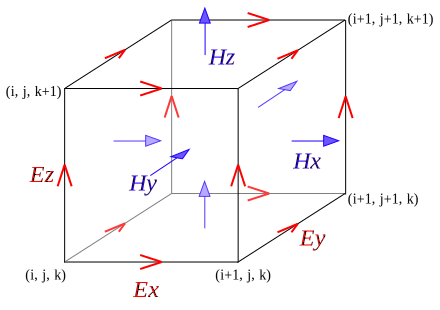
\includegraphics[width=75mm]{graphics/yee-cell}
\includegraphics[width=0.5\textwidth]{graphics/Yee-Cubes}
\caption{Поля в ячейке сетки Йе.
    Из таких ячеек составляется пространственная трехмерная сетка Йе, взаимодействие
    волн с веществом учитывается заданием в каждой ячейке значений диэлектрической
    и магнитной проницаемости и удельной проводимости.}
\label{fig:YeeCell}
\end{figure}
